\documentclass[11pt, oneside]{article} 
\usepackage{geometry}
\geometry{letterpaper} 
\usepackage{graphicx}
	
\usepackage{amssymb}
\usepackage{amsmath}
\usepackage{parskip}
\usepackage{color}
\usepackage{hyperref}

\graphicspath{{/Users/telliott_admin/Dropbox/Tex/png/}}
% \begin{center} 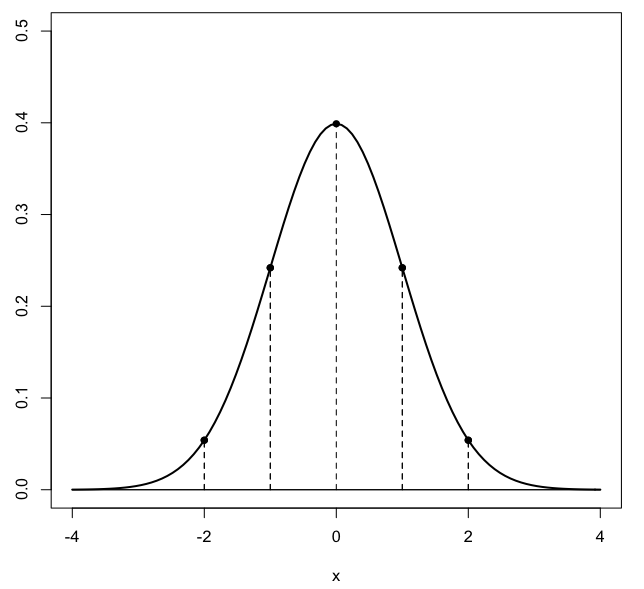
\includegraphics [scale=0.4] {gauss3.png} \end{center}

\title{Introduction}
\date{}

\begin{document}
\maketitle
\Large

The set $\mathbb{Q}$ (for quotient) are the rational numbers, derived from ratio.  Here is one definition, from Courant and Robbins.

\[ \mathbb{Q} = \{ \frac{p}{q} \} \text{ for } p \in \mathbb{Z}, q \in \mathbb{N} \]

Notice that we have defined $q > 0$.  If $p/q$ is to be less than zero, then it is enough that one of $p$ or $q$ be less than zero.  However, most authors don't make a big deal out of this, and will just say $p,q \in \mathbb{Z}$.

\subsection*{decimal representation}

Every rational number can be represented as a decimal, using the method known as long division.

Consider $1/2$
\[ 2 \overline{)1.000} \]
$2$ does not \emph{go into} $1$, but it does go into $10$ exactly $5$ times, giving $0.5$.  The remainder is zero and so the division process terminates.

Consider $1/8$.
\[ 8 \overline{)1.000} \]
$\circ$  $8$ goes into $10$ once, leaving $2$ as remainder

$\circ$  $8$ goes into $20$ twice, leaving $4$.  

$\circ$  $8$ goes into $40$ exactly $5$ times with no remainder.

The result is $0.125$.

The other possibility is that in going through the process a remainder comes up that has been seen previously.  

If we don't terminate with zero, then this must eventually happen, because there are only as many as $q$ possible remainders.

Thus, for example
\[ 1/7 = 0.142857142857 \dots \]

which contains $142857$, repeating forever.

\subsection*{decimals to fractions}

Conversely, every repeating decimal can be represented as a rational number.  For example

\[ 1 \times r = 0.142857142857 \dots \]
\[ 1000000 \times r = 142857.142857 \dots \]
\[ 999999 \times r = 142857 \]
\[ r = \frac{142857}{999999} = \frac{1}{7} \]
(since $142857$ goes into $999999$ exactly $7$ times).  

You can do this trick with 
\[ r = 0.333 \dots \]
\[ 10 \times r = 3.33 \dots \]
\[ 9 \times r = 3 \]
\[ r = \frac{3}{9} = \frac{1}{3} \]
or even
\[ r = 0.4999 \dots \]
\[ 10*r = 4.999 \dots \]
\[ 9*r = 4.5 \]
\[ r = \frac{4.5}{9} = \frac{1}{2} \]
and
\[ r = 0.9999 \dots \]
\[ 10*r = 9.999 \dots \]
\[ 9*r = 9 \]
\[ r = \frac{9}{9} = 1 \]

This is one of the subtleties of numbers.  In what sense can we say that 
\[ 0.5 = 0.4999 \dots \]
\[ 1 = 0.9999 \dots \]

Most everyone is OK with the example $1/3 = 0.3333 \dots$ but some may be uneasy with the other two.

Ultimately, we justify defining the result as coming from evaluation of a limit.  Consider $0.9999$.  For $n \in \mathbb{N}$, then as $n \rightarrow \infty$ the number being shown approaches $1$.  We'll come back to this after introducing the real numbers.

\subsection*{ordering}
For two rational numbers $a$ and $b$ there are only three cases:  either $a=b$, $a < b$ or $b < a$.

\[ \frac{p}{q} < \frac{s}{t} \ \iff \ pt < qs \]

$p/q$ is less than $s/t$ if and only if $pt < qs$.  Ordering of the integers guarantees ordering of the rational numbers.

Note:  we used the property that if
\[ a < b \]
then for $c > 0$
\[ ca < cb \]

\subsection*{density}
Consider the set of all points
\[ x = \frac{p}{10^n} \]
for all natural numbers $n$ and integers $p$.

It is clear that simply by increasing the value of $n$, we can construct a set of equally spaced rational numbers as tightly clustered as we wish.

The rational numbers are said to be \emph{dense} on the number line.  

$\bullet$  Between \emph{any} two rational numbers it is always possible to find another rational number.  

We describe this situation by writing that
\[ \forall \ u,v \in \mathbb{Q} \ \exists \ w \in \mathbb{Q} \ | \ w \in (u,v) \]
For every open interval whose bounds are rational numbers, there exists another rational number between $u$ and $v$.

\subsection*{example}
Suppose we have the numbers $p/q, s/t \in \mathbb{Q}$ and that $p/q < s/t$.  The average of is
\[ r = \frac{1}{2} \ [ \  \frac{p}{q} + \frac{s}{t} \ ] \ = \frac{pt+sq}{2qt} \]
Thus, $r$ is rational and is equal to the average of $p/q$ and $s/t$, so it lies between them.  

More formally, as $r$ is defined above, it has the property
\[ \frac{p}{q} < r < \frac{s}{t} \]
Proof:  substitute $p/q$ for $s/t$ in the equation of the average, defining $r$ above.  The resulting number is smaller than $r$, because the substituted value is smaller than $s/t$
\[ \frac{1}{2} \ [ \  \frac{p}{q} + \frac{p}{q} \ ] \ < \frac{1}{2} \ [ \  \frac{p}{q} + \frac{s}{t} \ ] \  = r \]
but the left-hand side is equal to $p/q$.  Now do the same thing with $s/t$.
\[ r = \frac{1}{2} \ [ \  \frac{p}{q} + \frac{s}{t} \ ] \ < \frac{1}{2} \ [ \  \frac{s}{t} + \frac{s}{t} \ ]  \]

\subsection*{intervals}
We denote the numbers greater than $u$ and less than $v$ as lying in the interval $(u,v)$.  With parentheses symbols, the interval described is \emph{open}, it does not include the boundary values.

To describe a \emph{closed} interval, write $[u,v]$.  This interval includes all the values in the first one, plus it also includes $u$ and $v$.

Because of the density property described above, an interval such as
\[ I = [0,1] \]
contains an infinite quantity of rational numbers.

\end{document}